%%%%%%%%%%%%%%%%%%%%%%%%%%%%%%%%%%%%%%%%%%%%%%%%%%%%%%%%%%%%%%%%%%%%%%
% LaTeX Template: Designer's CV
%
% Source: http://www.howtotex.com
% 
% Feel free to distribute this example, but please keep the referral
% to HowToTeX.com
% 
% Date: March 2012
%
% Modified by Lim Lian Tze to support multiple pages using fix provided at
% http://www.howtotex.com/templates/creating-a-designers-cv-in-latex/
% Date: November 2014
%%%%%%%%%%%%%%%%%%%%%%%%%%%%%%%%%%%%%%%%%%%%%%%%%%%%%%%%%%%%%%%%%%%%%%
% How to use writeLaTeX: 
%
% You edit the source code here on the left, and the preview on the
% right shows you the result within a few seconds.
%
% Bookmark this page and share the URL with your co-authors. They can
% edit at the same time!
%
% You can upload figures, bibliographies, custom classes and
% styles using the files menu.
%
% If you're new to LaTeX, the wikibook is a great place to start:
% http://en.wikibooks.org/wiki/LaTeX
%
%%%%%%%%%%%%%%%%%%%%%%%%%%%%%%%%%%%%%%%%%%%%%%%%%%%%%%%%%%%%%%%%%%%%%%

%%%%%%%%%%%%%%%%%%%%%%%%%%%%%%%%%%%%%
% Document properties and packages
%%%%%%%%%%%%%%%%%%%%%%%%%%%%%%%%%%%%%
\documentclass[a4paper,12pt,final]{memoir}

% misc
\renewcommand{\familydefault}{bch}	% font
\pagestyle{empty}					% no pagenumbering
\setlength{\parindent}{0pt}			% no paragraph indentation


% required packages (add your own)
\usepackage{flowfram}										% column layout
\usepackage[top=1cm,left=1cm,right=1cm,bottom=1cm]{geometry}% margins
\usepackage{graphicx}										% figures
\usepackage{url}											% URLs
\usepackage[usenames,dvipsnames]{xcolor}					% color
\usepackage{multicol}										% columns env.
	\setlength{\multicolsep}{0pt}
\usepackage{paralist}										% compact lists
\usepackage{tikz}

%%%%%%%%%%%%%%%%%%%%%%%%%%%%%%%%%%%%%
% Create column layout
%%%%%%%%%%%%%%%%%%%%%%%%%%%%%%%%%%%%%
% define length commands
\setlength{\vcolumnsep}{\baselineskip}
\setlength{\columnsep}{\vcolumnsep}

% left frame
\newflowframe{0.2\textwidth}{\textheight}{0pt}{0pt}[left]
	\newlength{\LeftMainSep}
	\setlength{\LeftMainSep}{0.2\textwidth}
	\addtolength{\LeftMainSep}{1\columnsep}
 
% small static frame for the vertical line
\newstaticframe{1.5pt}{\textheight}{\LeftMainSep}{0pt}
 
% content of the static frame
\begin{staticcontents}{1}
\hfill
\tikz{%
	\draw[loosely dotted,color=RoyalBlue,line width=1.5pt,yshift=0]
	(0,0) -- (0,\textheight);}%
\hfill\mbox{}
\end{staticcontents}
 
% right frame
\addtolength{\LeftMainSep}{1.5pt}
\addtolength{\LeftMainSep}{1\columnsep}
\newflowframe{0.7\textwidth}{\textheight}{\LeftMainSep}{0pt}[main01]


%%%%%%%%%%%%%%%%%%%%%%%%%%%%%%%%%%%%%
% define macros (for convience)
%%%%%%%%%%%%%%%%%%%%%%%%%%%%%%%%%%%%%
\newcommand{\Sep}{\vspace{1.5em}}
\newcommand{\SmallSep}{\vspace{0.5em}}

\newenvironment{AboutMe}
	{\ignorespaces\textbf{\color{RoyalBlue} About me}}
	{\Sep\ignorespacesafterend}
	
\newcommand{\CVSection}[1]
	{\Large\textbf{#1}\par
	\SmallSep\normalsize\normalfont}

\newcommand{\CVItem}[1]
	{\textbf{\color{RoyalBlue} #1}}


%%%%%%%%%%%%%%%%%%%%%%%%%%%%%%%%%%%%%
% Begin document
%%%%%%%%%%%%%%%%%%%%%%%%%%%%%%%%%%%%%
\begin{document}

% Left frame
%%%%%%%%%%%%%%%%%%%%
%
% Upload your own photo using the files menu
\begin{figure}
	\hfill
	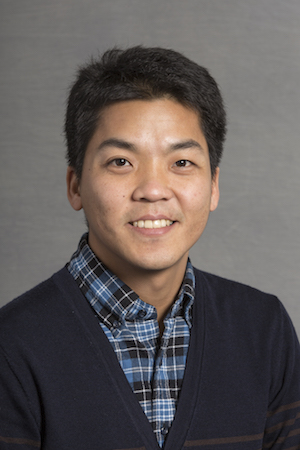
\includegraphics[width=0.8\columnwidth]{cr.jpg}
	\vspace{-6.5cm}
\end{figure}

\begin{flushright}\small
	Chaiyong Ragkhitwetsagul \\
	\url{ucabagk@ucl.ac.uk}  \\
    Department of Computer Science\\
    UCL, London\\
    WC1E 6BT

\end{flushright}\normalsize
\framebreak


% Right frame
%%%%%%%%%%%%%%%%%%%%
\Huge\bfseries {\color{RoyalBlue} Chaiyong Ragkhiwetsagul} \\
\Large\bfseries  Research Student \\
\small \url{www.cs.ucl.ac.uk/staff/C.Ragkhitwetsagul} \\

\normalsize\normalfont

% About me
\begin{AboutMe}
I am currently a 3rd year PhD student 
in Centre for Research on Evolution, Search and Testing (CREST), department of Computer Science at University College London. I am supervised by Dr. Jens Krinke and Dr. David Clark.
\newline \newline
I am also an assistant instructor at the Faculty of ICT, Mahidol University who is the main sponsor for my PhD study.
\newline \newline
I received a bachelor degree in Computer Engineering from Kasetsart University, Thailand and a master degree in MSIT--Very Large Information Systems (currently called Master of Computational Data Science) from Carnegie Mellon University, USA.
\end{AboutMe}

% Current projects
\CVSection{Current Projects}
\begin{compactitem}[\color{RoyalBlue}$\circ$]
	\item \CVItem{ISiCS}: Internet-scaled similar code search.
	\item \CVItem{Cloverflow}: A study of outdated code and license violation of reused code snippets between Stack Overflow and open source projects.
	\item \CVItem{CloPlag}: A comparison of code similarity analysers.
\end{compactitem}
\SmallSep

\CVSection{Publications}
C. Ragkhitwetsagul, J. Krinke, D.Clark (2017). \CVItem{A Comparison of Code Similarity Analysers.} UCL CS Research Notes No. RN/17/04, 2017. University College London, UK \vspace{2mm} \\
C. Ragkhitwetsagul, J. Krinke (2017). \CVItem{Using Compilation/Decompilation to Enhance Clone Detection.} In 11th International Workshop on Software Clones, 2017. Klagenfurt, Austria, To Appear --- \textbf{(The People's Choice Award Winner)} \vspace{2mm} \\
C.~Ragkhitwetsagul, M.~Paixao, M.~Adham, S.~Busari, J.~Krinke, and J.~H.~Drake (2016). \CVItem{Searching for Configurations in Clone Evalution: A Replication Study.} In 8th International Symposium on Search-based Software Engineering (SSBSE): Challenge Track, 2016. NC, USA. --- \textbf{(The NSF Student Travel Support)} \vspace{2mm} \\
C. Ragkhitwetsagul, J. Krinke, D. Clark (2016). \CVItem{Similarity of Source Code in the Presence of Pervasive Modifications.} In 16th IEEE International Working Conference on Source Code Analysis and Manipulation (SCAM), 2016. NC, USA. \vspace{2mm} \\
C. Ragkhitwetsagul (2016). \CVItem{Measuring Code Similarity in Large-scaled Code Corpora.} In 32nd International Conference on Software Maintenance and Evolution (ICSME): Doctoral Symposium, 2016. NC, USA. \vspace{2mm} \\
P. Janviriya, T. Ongarjithichai, P. Numruktrakul, C. Ragkhitwetsagul. (2014). \CVItem{CloudyDays : Cloud Storage Integration System.} In ICT-ISPC 2014 (pp. 125-128). Nakhonpathom, Thailand. \vspace{2mm} \\

% You'll need these 3 lines at the end of each page!
\clearpage
\framebreak
\framebreak

P. Hathaiwichian, L. Siriwittayacharoen, A. Wongwachirawanich, C. Ragkhitwetsagul (2014). \CVItem{Android Application for Event Management and Information Propagation.} In ICT-ISPC 2014 (pp. 139-142). Nakhonpathom, Thailand.
\SmallSep
\Sep

% Education
\CVSection{Education}
\CVItem{2014 - present, PhD}\\
\textbf{MPhil/PhD in Computer Science}\\
University College London, UK\\
Research topic: Code Similarity and Its Applications to Internet-scale Code Cloning
Supervisors: Dr. Jens Krinke, Dr. David Clark\\
Research interest: clone detection, source code plagiarism detection, code similarity, mining of software repository, SBSE
\SmallSep

\CVItem{2007 - 2008, Master}\\
\textbf{MSIT - Very Large Information Systems}\\
Carnegie Mellon University, USA\\
Capstone project: Honeydew: Predicting meeting date using machine learning algorithm

\SmallSep

\CVItem{2002 - 2005, Undergraduate}\\
\textbf{Bachelor Degree in Computer Engineering (Magna cum Laude)}\\
Kasetsart University, Thailand
\SmallSep
\Sep

% Achievements
\CVSection{Achievements/Awards}
\begin{tabular}{lp{11.5cm}}
	
	\CVItem{2017} & The People's Choice Award for\newline \textit{Using Compilation/Decompilation to Enhance Clone Detection}\newline at IWSC 2017. Klagenfurt, Austria. \\
	\CVItem{2016} & NSF Student Travel Support (700 USD) for SSBSE 2016. Raleigh, NC, USA. \\
	\CVItem{2016} & Microsoft Azure Research Award (\$20,000 cloud computing) for the ISiCS: Internet-scaled Similar Code Search project \\ 
	\CVItem{2014} & Mahidol University’s Academic Development Scholarship \\
	\CVItem{2014} & Faculty of ICT, Mahidol University PhD scholarship \\
	\CVItem{2008} & Best Project Award: 15-637 Web App Development, CMU, 2008 \\
	\CVItem{2007} & The Royal Thai Government scholarship \\
	\CVItem{2006} & National Software Contest of Thailand (NSC): Winner in software for entertainment category \\ 
	\CVItem{2005} & DTAC \& NOKIA i-Awards mobile app contest: finalists
\end{tabular} 
\SmallSep
\Sep

% Experience
\CVSection{Experience}
\CVItem{Sep 2014 - Present, Research Student (PhD candidate)}\\
\textbf{Department of Computer Science, University College London}\\
A member of Centre for Research on Evolution, Search and Testing (CREST) under Software Systems Engineering (SSE) group. \\

% You'll need these 3 lines at the end of each page!
\clearpage
\framebreak
\framebreak

\CVItem{Dec 2012 - Sep 2014, Assistant Instructor}\\
\textbf{Faculty of ICT, Mahidol University, Nakhonpathom, Thailand}\\
A lecturer of Fundamentals of Programming, OOP, DBMS, Knowledge-based Systems, Android App Development.\\ 
A researcher in Mahidol University Electronic Research Information System (MU eRIS) project, and advising 3 undergraduate senior projects.

\SmallSep

\CVItem{Nov 2011 - Sep 2014, Consultant}\\
\textbf{Blaccess Thailand}\\
Making key decisions and providing company's vision.\\
Planning and managing IT projects and staffs.

\SmallSep

\CVItem{Jan 2009 - Nov 2012, System Analyst}\\
\textbf{National Economic and Social Development Board, Thailand}\\
Planning, migrating, and developing new NESDB IT services (email system, web applications, databases, and networks).\\
IT consultant and network administrator.

\SmallSep

\CVItem{Feb 2010 - Dec 2012, Teacher}\\
\textbf{ProGaming, Thailand}\\
Instructing the Pro Android course focusing on how to develop an Android application.\\
Instructing the Pro iOS course focusing on how to develop an iOS application.

\SmallSep

\CVItem{Jan 2009 - Dec 2012, Research Assistant}\\
\textbf{Kasetsart University, Thailand}\\
Developing a digital repository, training and project tracking system for Puparn Royal Development Study Center.
\SmallSep

\CVItem{Mar 2008 - Aug 2008, Intern}\\
\textbf{Oracle, USA}\\
Developing a new version of testing platform called Distributed\\ 
Testing System (DTS) using Java Servlet, JSP, and Javascript.

\SmallSep

\CVItem{Feb 2006 - Apr 2007, Software Test Engineer}\\
\textbf{Microsoft, Thailand}\\
Creating automated test tools for testing localized versions of Windows Vista User Assistance Platform.\\
Testing user assistance (UA) contents in XML format.

\SmallSep
\Sep

% Skills
\CVSection{Skills}
\CVItem{Platforms}
\begin{multicols}{2}
\begin{compactitem}[\color{RoyalBlue}$\circ$]
	\item Mac
    \item Linux
    \item Windows
    \item Raspberry Pi
    \item iOS
    \item Android
\end{compactitem}
\end{multicols}
\SmallSep

\CVItem{Computer programming}
\begin{multicols}{2}
\begin{compactitem}[\color{RoyalBlue}$\circ$]
	\item Java
    \item C/C++
	\item Obj-C 
	\item .Net 
	\item HTML
	\item PHP
	\item SQL
\end{compactitem}
\end{multicols}
\Sep 

% References
\CVSection{References}
References upon request.

%%%%%%%%%%%%%%%%%%%%%%%%%%%%%%%%%%%%%
% End document
%%%%%%%%%%%%%%%%%%%%%%%%%%%%%%%%%%%%%
\end{document}